% TODO:


\documentclass[12pt, a4paper]{scrartcl}

\usepackage{graphicx}
\usepackage[ngerman]{babel}
\RequirePackage[ngerman=ngerman-x-latest]{hyphsubst}
\usepackage[utf8]{inputenc}
\usepackage[T1]{fontenc}
\usepackage[autostyle,german=guillemets]{csquotes}
\usepackage{verbatim}
\usepackage[singlespacing, onehalfspacing]{setspace}
\usepackage{lmodern}
\usepackage{pdfpages} % gut für Anhänge!
\usepackage{apacite}
\usepackage{url}
\usepackage{enumitem}
\usepackage{pdflscape}
%\usepackage{tabularx}
\usepackage{blindtext}
\usepackage{lipsum}
%\usepackage{relsize}
\usepackage{tocstyle}
\usepackage{color, colortbl}
%\usepackage[all]{nowidow}
\usepackage[pagewise]{lineno}
\usepackage{longtable}



\begin{document}

\title{Unterrichtsentwurf für eine Lehrprobe im Fach Politik}
\author{Dr. Hendrik Bunke}
\date{}
\thispagestyle{empty}

%\maketitle
\begin{center}
{
\includegraphics[height=1.1cm]{lis.png}}
\singlespacing
{\Huge
    {\textsf
        {\textbf{Unterrichtsentwurf für eine Lehrprobe im Fach Politik}
        }
    }
}

\vspace{0.5cm}
\Large{Dr. Hendrik Bunke}



\end{center}



% !TEX root = 0.gesamt.tex



\singlespacing

\small
\begin{center}
\begin{tabular}{llllll}

\textbf{Schule:} & Datenschutz &
\textbf{Klasse:} & Datenschutz &
\textbf{Raum:} & Datenschutz \\
\textbf{Datum:}  & 01.04.2019  &
\textbf{Zeit:} & 11:45-12:30 Uhr &&\\


\\

\end{tabular}
%\begin{center}
\begin{tabular}{p{6cm}p{9cm}}
    \textbf{Thema der Unterrichtsstunde:}& Wahlbeteiligung als sozialstrukturelles Problem \\
    \textbf{Thema der Unterrichtseinheit:}& Wahlen, Wähler und Wahlkampf am  Beispiel der Bremer Bürgerschaftswahl 2019\\


\end{tabular}

\end{center}

\section*{Prüfungskommission}

\begin{tabular}{p{6cm} p{6cm}}
    \textbf{Vorsitzende:}& Datenschutz\\
    \textbf{Fachleiter Politik:} & Datenschutz\\
    \textbf{Fachleiterin Sport:} & Datenschutz\\
    \textbf{Fachleiterin BW:} & Datenschutz\\
    \textbf{Schulvertreterin:} & Datenschutz\\ 
    \textbf{Vertrauensreferendarin:} & Datenschutz\\

\end{tabular}





\normalsize


\footnotesize
\renewcommand{\contentsname}{Gliederung}
\usetocstyle{classic} %bewirkt, dass die Seitenzahlen genauso wie die Title formatiert sind (Größe!)
\tableofcontents

\newpage
\setcounter{page}{1}
% \onehalfspacing
\normalsize

% LIS Vorgabe ist 28-31 Zeilen pro Seite, weswegen das erheblich schönere
% \onehalfspacing von LaTeX nicht geht, damit wären's so rund 35. Keine Ahnung,
% ob das ein Problem wäre, aber sicher ist sicher
\setstretch{1,33}

%\linenumbers   % Zeilennummern um zu testen
%\modulolinenumbers[5]

% !TEX root = 0.gesamt.tex

\section{Lerngruppe und Unterrichtssituation}

\emph{Dieser Teil wurde aus Datenschutzgründen für die Veröffentlichung entfernt}

\subsection{Rahmenbedingungen}


\subsection{Interaktionsbeziehungen}


\subsection{Kompetenzorientierte Lern- und Unterrichtsvoraussetzungen und erste Konsequenzen}

% !TEX root = 0.gesamt.tex

% background color for special row in unterrichtssequenz
\definecolor{Gray}{gray}{0.9}


\section{Einordnung des Themas in curriculare Vorgaben und die Unterrichtssequenz}

Die geplante Unterrichtsstunde ist Teil der UE \emph{Wahlen, Wähler und
Wahlkampf am  Beispiel der Bremer Bürgerschaftswahl 2019}, die sich einordnet
in den im Bremer Bildungsplan für Politik in der 10. Klasse genannten
Themenbereich \enquote{Gesellschaftliche Realität(en)} und die dort
aufgeführten Inhalte \enquote{Demokratie als Gesellschaftsprinzip und
Gesellschaftliche Kräfteverhältnisse} und \enquote{Sozialstruktur,
demografische Entwicklungen und deren Auswirkungen} \cite[S.
35]{dersenatorfurbildungundwissenschaft2006}. Im schulinternen Curriculum wird
unter dem o.g. Themenbereich explizit das in der UE behandelte Thema
\enquote{Wahlen, Wähler und Wahlkampf} konkretisiert. Innerhalb der Unterrichtseinheit folgt das
behandelte Thema \emph{Wahlbeteiligung} auf zwei eher wissensorientierte
Stunden (Wahlamt, \enquote{Wissen wie Wählen}), die ausgingen von konkreten
Fragen der SuS, sowie einer eher theoretischen Auseinandersetzung mit der
Funktion von Wahlen in Demokratien. Im zweiten Teil der UE folgt die
Auseinandersetzung mit Inhalten, Parteiprogrammen und Wahlkampfthemen der
Bremer Bürgerschaftswahl sowie zum Abschluss die Analyse des Wahlergebnisses.


\subsection{Unterrichtssequenz}

\begin{footnotesize}

\begin{tabular}{|p{2cm}|p{12.75cm}|}
\hline
\textbf{Stunde} & \textbf{Inhalt}  \\
\hline
1 & Einstieg und Themenerarbeitung \\
\hline
2 & Exkursion Wahlamt \\
\hline
3 & WWW - Wissen Wie Wählen \\
\hline
4 & Wahlen und Demokratie \\
\hline
\rowcolor{Gray}
\textbf{5} & \textbf{Wahlbeteiligung als sozialstrukturelles Problem} \\
\hline
6 & Parteien und Wahlprogramme \\
\hline
7 & Wahlkampf: Themen, Analysen, Prognosen \\
\hline
8 & Wahlanalyse und UE Auswertung\\
\hline

\end{tabular}

\end{footnotesize}

\vspace{0.5cm}

% !TEX root = 0.gesamt.tex
\section{Sachanalyse}

An den letzten Bürgerschaftswahlen im Land Bremen im Jahr 2015 beteiligten sich
lediglich 50,2\% der Wahlberechtigten, d.h. von knapp 488.000 Wahlberechtigten
nahmen nur gut 244.000  \cite<vgl. das amtliche Endergebnis in>[S.
7]{wayand2015} dieses Recht in Anspruch. Damit setzte sich ein seit 1987 in
Bremen zu verzeichnender Trend sinkender Wahlbeteiligung fort \cite[S.
10]{wayand2015}. Bei keiner Bürgerschaftswahl seit 1946 war die Wahlbeteiligung
niedriger. Besonders drastisch fiel dabei auch das nochmalige Absinken um 5,3
Prozentpunkte gegenüber der vorhergehenden Wahl von 2011 aus \cite[S.
11]{wayand2015}. Dabei ist der Trend sinkender Wahlbeteiligung zwar ein
bundesweiter, allerdings fällt er in Bremen besonders stark aus. In keinem
westlichen Bundesland gab es seit 1946 eine niedrigere Wahlbeteiligung bei
Landtagswahlen \cite[S. 7]{vehrkamp2015}.

Mit der Wahlbeteiligung sinkt auch die \emph{Repräsentationsquote} drastisch.
Der aktuelle rot-grüne Senat repräsentiert nur noch rund 23\% der
Wahlberechtigten. Rechnet man die nicht wahlberechtigten Ausländer hinzu, sinkt
die Repräsentationsquote des Senats sogar auf unter 20\%, die der Bürgerschaft
(Landtag) auf 41,6\%.

Schon diese geringe Repräsentationsquote ist ein prinzipielles Problem für eine
repräsentative Demokratie. \enquote{Hinter der regierenden Mehrheit steht dann
unter Umständen nur noch eine zahlenmäßig kleine Minderheit} \cite{decker2016},
was unmittelbar die Frage nach der demokratischen Legitimation von Parlament
und Regierung aufwirft. Diese Frage wird noch dringender, betrachtet man die
steigende \emph{soziale Selektivität} der Wahlbeteiligung \cite<vgl. hierzu
ausführlich>{schafer2015, decker2016, vehrkamp2015, schafer2013}. Hier
konstatiert die Forschung einen eindeutigen Befund. \enquote{Die soziale Lage
eines Ortsteils bestimmt die Höhe der Wahlbeteiligung: Je höher der Anteil von
Haushalten aus den sozial schwächeren Milieus, je höher die Arbeitslosigkeit,
je geringer der formale Bildungsstand und je geringer die durchschnittliche
Kaufkraft der Haushalte in einem Ortsteil, desto geringer ist die
Wahlbeteiligung} \cite[S. 9]{vehrkamp2015}. Dies gilt nicht nur für Bremen,
sondern für ganz Deutschland, besonders die Großstädte \cite{schafer2013,
schafer2015}. Hintergrund der geringen Wahlbeteiligung ist also die soziale
Spaltung der Wählerschaft. Wissenschaft \cite{vehrkamp2015, schafer2013} und
auch Politik\footnote{ Siehe z.B. das Interview mit dem Vorsitzenden der
SPD"~Fraktion in der Bremischen Bürgerschaft im Weser"~Kurier vom 30.01.2019
\cite{boekhoff2019}.} sprechen inzwischen von \emph{prekären Wahlen}. Es
entsteht ein selbsteskalierender Prozess: Wahlenthaltung führt zu mangelnder
Interessenvertretrung im Parlament, wodurch Nichtwähler wiederum noch weniger
Gründe haben, zur Wahl zu gehen \cite{decker2016}. Die sinkende
Repräsentationsquote betrifft also vor allem die sozial benachteiligten
Wählergruppen und Stadtteile und ist damit nicht nur ein prinzipielles
Legitimations-Problem, sondern auch und vor allem ein sozialstrukturelles.

% !TEX root = 0.gesamt.tex
\section{Didaktische Analyse}

Die SuS setzen sich in der geplanten Stunde mit dem Zusammenhang zwischen
Wahlbeteiligung und Sozialstruktur auseinander und beurteilen die daraus
entstehenden Probleme für die repräsentative Demokratie. Dies geschieht anhand
der Bremer Bürgerschaftswahl 2015 sowie anlässlich der Bürgerschaftswahl 2019,
bei der viele der SuS zum ersten Mal wählen dürfen. Folgt man den Prinzipien
der didaktischen Analyse von \citeA{klafki1962}, ergibt sich hieraus
unmittelbar die \textbf{Gegenwartsbedeutung} der gesamten UE wie auch der
geplanten Stunde. Die Auseinandersetzung mit Funktion, Ablauf, Inhalten und
Problemen von Wahlen als einem wesentlichen Pfeiler der repräsentativen
Demokratie ist für die SuS unmittelbar bedeutsam und fördert ihre
\textbf{politische Handlungsfähigkeit}. Diese Bedeutung wurde auch deutlich
anhand der vielen Fragen der SuS anlässlich des Einstiegs, die für den weiteren
Verlauf der UE die Grundlage bilden. Auch die Auseinandersetzung mit dem Thema
der geplanten Stunde ist für die SuS unmittelbar individuell bedeutsam, schon
alleine durch die ihnen bevorstehende prinzipielle Entscheidung, ob sie
überhaupt wählen gehen \textit{wollen}.\footnote{Bei einer in der
Einstiegsstunde anonym durchgeführten \enquote{Sonntagsfrage} (\emph{Was
würdest Du wählen, wenn am kommenden Sonntag Wahl wäre?}) entschieden sich
sechs von 25 SuS für Nichtwahl.} Im Rahmen ihrer Rolle als Bürger im System der
repräsentativen Demokratie werden diese Fragen auch in absehbarer Zukunft für
die SuS bedeutsam sein (\textbf{Zukunftsbedeutung}). Mit diesem
\emph{persönlichen Bezug} ist eine Ebene der \textbf{Struktur des Inhalts}
bereits skizziert. Eine weitere Ebene stellt die soziale Selektivität der
Wahlbeteiligung dar, mit der gleichzeitig die soziale Ungleichheit von
Stadtteilen in Bremen (und anderen Großstädten) thematisiert ist
(\textbf{politische Analysefähigkeit}). Die dritte Ebene thematisiert die Frage
nach der aus der \emph{sozialen Selektivität} resultierenden faktisch nicht
mehr vorhandenen \emph{sozialen Repräsentativität} von Wahlergebnissen und den
Konsequenzen (\textbf{politische Urteilsfähigkeit}). Das \textbf{Entwerfen} und
\textbf{Diskutieren} von Lösungsvorschlägen ist eine vierte Ebene der
inhaltlichen Struktur, die die SuS aber eigenständig schriftlich bearbeiten
(Hausaufgabe).

Die Fokussierung auf die lokalen Bremer Wahlen ist zum einen lebensweltlich
begründet (Lebensumfeld der SuS), zum anderen werden die bundesweiten Probleme
der sinkenden Wahlbeteiligung, der sozialen Selektivität und den daraus
resultierenden Fragen nach Repräsentativität und der demokratischen
Legitimation von Regierung und Parlament hier, wie die Sachanalyse gezeigt hat,
besonders deutlich. Es handelt sich um ein generelles Problem des Systems der
repräsentativen Demokratie in Deutschland, welches sich anhand der Bremer
Bürgerschaftswahlen und Stadtteilstruktur beispielhaft erschließen lässt
(\textbf{exemplarische Bedeutung}). Die \textbf{Zugänglichkeit} des Themas wird
dabei zum einen über den persönlichen Bezug (ausgehend von der Reflexion des
eigenen Wahlverhaltens), zum anderen über den lokalen Bezug zum eigenen
Lebensumfeld (Bremen, eigenes Stadtviertel) ermöglicht.

% !TEX root = 0.gesamt.tex

\section{Kompetenzen}

% muss hier eigentlich nicht rein?  \subsection{Leitidee der Unterrichtsstunde}

% \subsection{Kompetenzraster}

\scriptsize
\begin{singlespacing}

\begin{longtable}{p{1.5cm}|p{2cm}|p{4cm}|p{4cm}|p{3cm}}

\hline
\textbf{Kompetenz Dimension} &

\textbf{Allgemeine fachspezifische Kompetenzbereiche} &

\textbf{Standards der Bildungspläne \newline \newline die SuS können...} &

\textbf{Aufgabenstruktur (Per"-formanz) \newline \newline ...indem sie...} &

\textbf{Differenzierte Kompetenz"-niveaus}

\\
\hline

\textbf{Fach"-kompetenz} &
Politische Analysefähig"-keit

Politische Urteilsfähigkeit

Politische Handlungsfähigkeit

&
...aktuelle politische Prozesse auf demokratische Kernprinzipien analysieren und gesellschaftliche Machtverhältnisse und Interessensgegensätze reflektieren...,

...das gesellschaftliche System im Hinblick auf soziale Strukturen an ausgewählten Beispielen beschreiben und erklären...,

...grundlegende gesellschaftliche Herausforderungen unter dem Gesichtspunkt sozialer Gerechtigkeit benennen und erklären sowie an ausgewählten Beispielen gesellschaftliche Entwicklungen beschreiben und die damit zusammenhängenden Probleme benennen...,
&

...die sich aus der niedrigen Wahlbeteiligung ergebenden Probleme \textbf{benennen} und \textbf{beschreiben}

...in Arbeitsgruppen aus den gegebenen Teilstatistiken den Zusammenhang zwischen Wahlbeteiligung und Sozialstruktur \textbf{herausarbeiten}

...die niedrige Wahlbeteiligung unter dem Aspekt der sozialen Selektivität und der Repräsentationsquote des Parlaments \textbf{beurteilen}

...erste eigene Lösungsvorschläge für das Problem der geringen Wahlbeteiligung \textbf{entwerfen} (Hausaufgabe)
&
- die Statistiken eigenständig analysieren \newline
- die Statistiken mit Hilfestellung analysieren \newline


\\
\hline
\textbf{Methoden"-kompetenz} &

Erschließung von Informationen

Anwendung erschlossener Informationen

Problemlösungs- und
Argumentationsfähigkeit

&

...Informationen aus unterschiedlichen Quellen entnehmen, problemangemessen auswerten und in Zusammenhänge einordnen,

...Arbeitsergebnisse angemessen (u.a. mit Hilfe
moderner Medien) präsentieren.


&

...in Arbeitsgruppen aus den gegebenen Teilstatistiken den Zusammenhang zwischen Wahlbeteiligung und Sozialstruktur \textbf{herausarbeiten}

... die Arbeitsergebnisse in einem Satz schriftlich \textbf{zusammenfassen}, der Klasse \textbf{präsentieren} und \textbf{erläutern}

& % hier noch Differenzierung?
- diskutieren und formulieren (Gruppe) \newline
- präsentieren und erläutern (Referent*in der Gruppe)

\\
\hline
\textbf{Sozial"-kompetenz} &
Teamfähigkeit

Kommunikations"-fähigkeit

& % Bildungspläne leer, da steht nix über Sozialkompetenz :-)

&
...in der Gruppe gemein"-sam einen statistischen Sachverhalt erarbeiten und gemeinsam formulieren

& % hier noch Differenzierung?
- verbal diskutieren \newline
- ausschließlich schriftliche Formulierung

\\
\hline

\textbf{Personal"-kompetenz} &
Logisches Denken

Lernbereitschaft
&  % keine personalen Kompetenzen in den Bildungsplänen
&
...aus den gegebenen Teilstatistiken den Zusammenhang zwischen Wahlbeteiligung und Sozialstruktur \textbf{herausarbeiten}

...sie Interesse an zahlreichen, auch statistischen, neuen Informationen zeigen und sich dieses Wissen schnell aneignen
&

\\
\hline
\textbf{Sprach"-kompetenz}
& % keine allgemeinen Kompetenzen
& % keine Bildungsstandards
&
... Fachbegriffe präzise einsetzen können

... einen aus statistischen Materialien erarbeiteten Zusammenhang in einem Satz formulieren können

&

\\
\hline

\end{longtable}



\end{singlespacing}
\normalsize

% !TEX root = 0.gesamt.tex

\section{Methodische Überlegungen}

Basierend auf den didaktischen Überlegungen wird zunächst mit dem
\textbf{Einstieg} versucht, ein Problem zu benennen und ein allgemeines
\emph{Problembewusstsein} zu schaffen \cite[S. 427]{greving2014}. Dies
geschieht zunächst mit der Neugier und frageweckenden \cite{meyer1990}
Beamer-Projektion der \enquote{reinen} (kein \% Zeichen, kein weiterer Text)
Zahl der Beteiligungsquote der Bürgerschaftswahl von 2015 (50,2) an das
Smartboard, verbunden mit der Frage: Was könnte diese Zahl in unserem Kontext
bezeichnen? Nach der Klärung wird die Zahl von mir kurz ergänzt mit dem Verlauf
der Wahlbeteiligung in Bremen seit 1983 sowie der Information, dass dies ein
bundesweites Problem ist, das in Bremen besonders stark ausfällt. Die
Problematisierung der geringen Wahlbeteiligung wird mit der Frage eingeleitet,
ob und wenn ja warum aus der Sicht der SuS die geringe Wahlbeteiligung
überhaupt ein Problem darstellt (\textbf{Leitfrage}). Die Frage knüpft dabei an
die vorhergehende Stunde, in der die SuS sich mit der grundlegenden Bedeutung
von Wahlen für Demokratie beschäftigt haben. Die Antworten werden
stichpunktartig an der Tafel gesichert und führen hin zur Fokussierung des
Begriffs der allgemeinen \emph{Repräsentationsquote}. Die Bedeutung des
Begriffs wird durch die Einblendung einer Grafik visualiert.

Daraus entsteht die Leitfrage der \textbf{Erarbeitungsphase}: wer sind
eigentlich die Nichtwähler? Kann man sie bestimmten Sozialindikatoren zuordnen?
Hier nennen die SuS zunächst denkbare Indikatoren, von denen schließlich von
mir ausgewählte (die Auswahl folgt aus dem vorhandenen statistischen Material)
von den SuS in Gruppen bearbeitet werden sollen. Die Zusammenstellung der
Gruppen wird von mir vorab geplant und erfolgt leistungsheterogen, um zu
gewährleisten, dass alle Gruppenergebnisse qualitativ vergleichbar sind. Jede
Gruppe erhält ein Arbeitsblatt, in denen statistisch jeweils ein Indikator
(Arbeitslosigkeit, Wohnraum, Milieu, Bildung, Alter und Geschlecht) %falsch! Alter bezieht sich nicht auf die Ortsteile!
in Bezug
zur Wahlbeteiligung in den zehn Ortsteilen mit der höchsten und den zehn
Ortsteilen mit der niedrigsten Wahlbeteiligung gesetzt wird. Aufgabe für die
SuS ist es, anhand der gegebenen statischen Zahlen den Zusammenhang zwischen
Wahlbeteilung und Sozialstruktur zu analysieren und in maximal zwei Sätzen zu
formulieren. % Hilfekarten?
Der zuvor selbstbestimmte Schriftführer der Gruppe notiert das Ergebnis in einem vorbereiteten Padlet.\footnote{Den SuS ist
das Online Tool Padlet (\url{https://padlet.com}) aus früheren Stunden bekannt
und dient hier als interaktive digitale Tafel, die ein hohes Maß an
Interaktion, Schüleraktivität und nachhaltiger Ergebnissicherung bietet. Die
Notierung erfolgt per Smartphone, das im Politikunterricht als Recherche- und
Kollaborationstool für unterrichtliche Zwecke genutzt wird.} Anschließend
stellt jede Gruppe kurz erläuternd ihr Ergebnis vor, so dass schließlich die
soziale Selektivität als Gesamtbild erarbeitet, deutlich visualiert und
formuliert im Padlet am Smartboard steht (\textbf{Austausch- und
Sicherungsphase}). Dem Gesamtergebnis folgt die Notierung des Fachbegriffs der
\emph{sozialen Selektivität}, der das erarbeitete Ergebnis der SuS bezeichnet.

Damit ist die Leitfrage der Erarbeitungsphase beantwortet und festgehalten. In
der anschließenden \textbf{Transfer- und Diskussionsphase} wird zurückgegriffen
auf die im Einstieg nur prinzipiell problematisierte geringe
Repräsentationsquote des Wahlergebnisses, der Bürgerschaft und des Senats. Hier
wird die \textbf{Problematisierung} nun -- initiiert durch eine entsprechende
Eingangsfrage sowie einer Visualisierung durch die Verbindung der Begriffe
\emph{Repräsentationsquote} und \emph{soziale Selektivität} an Tafel und/oder
Smartboard -- vertieft und zusammengeführt mit dem Aspekt der sozialen
Selektiviät. Wahlbeteiligung wird als sozialstrukturelles Problem beurteilt und
diskutiert. Auf dieser Grundlage sollen die SuS in einer Hausaufgabe
Lösungsmöglichkeiten entwerfen und ggf. recherchieren (Vertiefung der
politischen  Urteils- und Handlungsfähigkeit).

Als \textbf{didaktische Reserve} dient die Diskussion der in der Debatte um die
niedrige Wahlbeteiligung vorgeschlagene Einführung einer Wahlpflicht \cite<vgl.
z.B.>[S. 207ff.]{kaeding2017, neu2017, schafer2015}.\footnote{Auch der damalige
Präsident der Bremischen Bürgerschaft, Christian Weber, sprach sich 2017 für
eine Wahlpflicht aus \cite{weber2017}.}

% !TEX root = 0.gesamt.tex

 % \newcolumntype{L}[1]{>{\raggedright\arraybackslash}p{#1}} % linksbündig mit Breitenangabe

 \begin{landscape}
 %\thispagestyle{empty}
 \section{Verlaufsplan}

 \singlespacing
 \scriptsize
 \begin{tabular}{p{2cm}|p{4.5cm}|p{4.5cm}|p{1.5cm}|p{2cm}|p{4.5cm}}

\textbf{Phase} &
\textbf{Aktivität Lehrkraft} &
\textbf{Aktivität SuS} &
\textbf{Sozialform} &
\textbf{Medien, Material} &
\textbf{didaktisch-methodischer Kommentar}

\\
\hline
% Begrüßung??
\textbf{Einstieg}
&
- begrüßt die SuS stellt die Kommission vor

- präsentiert am Smartboard die Zahl 50,2

- Frage: \emph{was könnte diese Zahl im Kontext der UE bezeichnen?}

- nennt und notiert das Thema der Stunde an der Tafel
&
- begrüßen L und die Kommission

- nennen mögliche Bedeutungen der Zahl
&
Plenum / UG
&
Smartboard, PC, Tafel
&
- Fokussierung, Neugier

- bei Bedarf werden Hilfestellungen eingeblendet

\begin{comment}
\begin{itemize*}
    \item bereitet vor und mit längerem text, aber das kostet zuviel platz

    \item kontrolliert
\end{itemize*}
\end{comment}

\\
\hline

\textbf{Problemati"-sierung I}
&
Leitfrage: \emph{Warum ist die geringe Wahlbeteiligung überhaupt ein Problem?}

- Sammelt Antworten stichpunktartig an der Tafel

- Präsentation des \enquote{wahren} Wahlergebnisses

- Einführung und Visualisierung des Begriffs \emph{Repräsentationsquote}
&
äußern Vermutungen und begründete Hypothesen
&
UG
&
Smartboard, PC, Tafel
&
- Problematisierung auf Grundlage der Ergebnisse aus der vorhergehenden Stunde

- (Fach)-Sprachkompetenz

\\
\hline

\textbf{Erarbeitung}
&
- teilt die Gruppen ein und verteilt Arbeitsblätter

- zeigt das vorbereitete Padlet und erläutert die Aufgabenstellung
&
- bearbeiten die Aufgabe

- Schriftführer notieren die Ergebnisse im Padlet
&
GA
&
Smartboard, PC, Arbeitsblätter, Smartphones, Padlet
&
leistungshetero"-gene Gruppeneinteilung (Diff"-erenzierung)

\\
\hline

\textbf{Austausch, Sicherung}
&
- ergänzt und korrigiert ggf.

- notiert zusammenfassendes Endergebnis im Padlet

- führt den Begriff \emph{soziale Selektivität} (und ergänzend den Begriff {\emph{prekäre Wahlen}) ein und notiert ihn als Oberbegriff im Padlet
&
- Gruppensprecher*innen präsentieren und erläutern die Ergebnisse

- fragen nach
&
UG, Schülerpräsentation
&
Smartboard, Padlet
&

\\
\hline

\textbf{Problemati"-sierung II}
&
Frage: \emph{Was bedeutet die soziale Selektivität für die Repräsentationsquote?}
&
- diskutieren und erörtern

- formulieren den Zusammenhang und die daraus resultierenden Probleme von sozialer Selektivität und Repräsentation
&
UG, Plenum
&
&
Vertiefung von Problematisierung I

\\
\hline


\textbf{Hausaufgabe}
&
erläutert, zeigt die Hausaufgabe auf itslearning
&
entwerfen Lösungsvorschläge vor dem Hintergrund der in der Stunde aufgezeigten Problematik und recherchieren ggf. dazu.
&
EA
&
&
- Abgabe erfolgt über itslearning

- Diskussion der Lösungsvorschläge in nachfolgender Stunde

\\
\hline

\textbf{Didaktische Reserve}
&
bitte um Stellungnahme zu dem Vorschlag, eine Wahlpflicht einzuführen
&
- nehmen Stellung und beurteilen eine mögliche Wahlpflicht
&
Plenum
&
&
Vorgriff auf Hausaufgabe

\end{tabular}

 \normalsize
 \onehalfspacing
 \end{landscape}



%\newpage

\pagestyle{empty}
\singlespacing
\bibliography{zotero.bib}
\bibliographystyle{apacite}

\newpage
\section*{Erklärung}
Diese schriftliche Planung habe ich selbstständig angefertigt. Andere als die
angegebenen Hilfsmittel habe ich nicht benutzt. Die Stellen der schriftlichen
Ausarbeitung, die anderen Werken, auch eigenen oder fremden unveröffentlichten
Prüfungsarbeiten, im Wortlaut oder ihrem wesentlichem Inhalt nach entnommen
sind, habe ich mit genauer Angabe der Quelle kenntlich gemacht.

\vspace{1cm}Bremen, 29.03.2019

\vspace{3cm}(Dr. Hendrik Bunke)



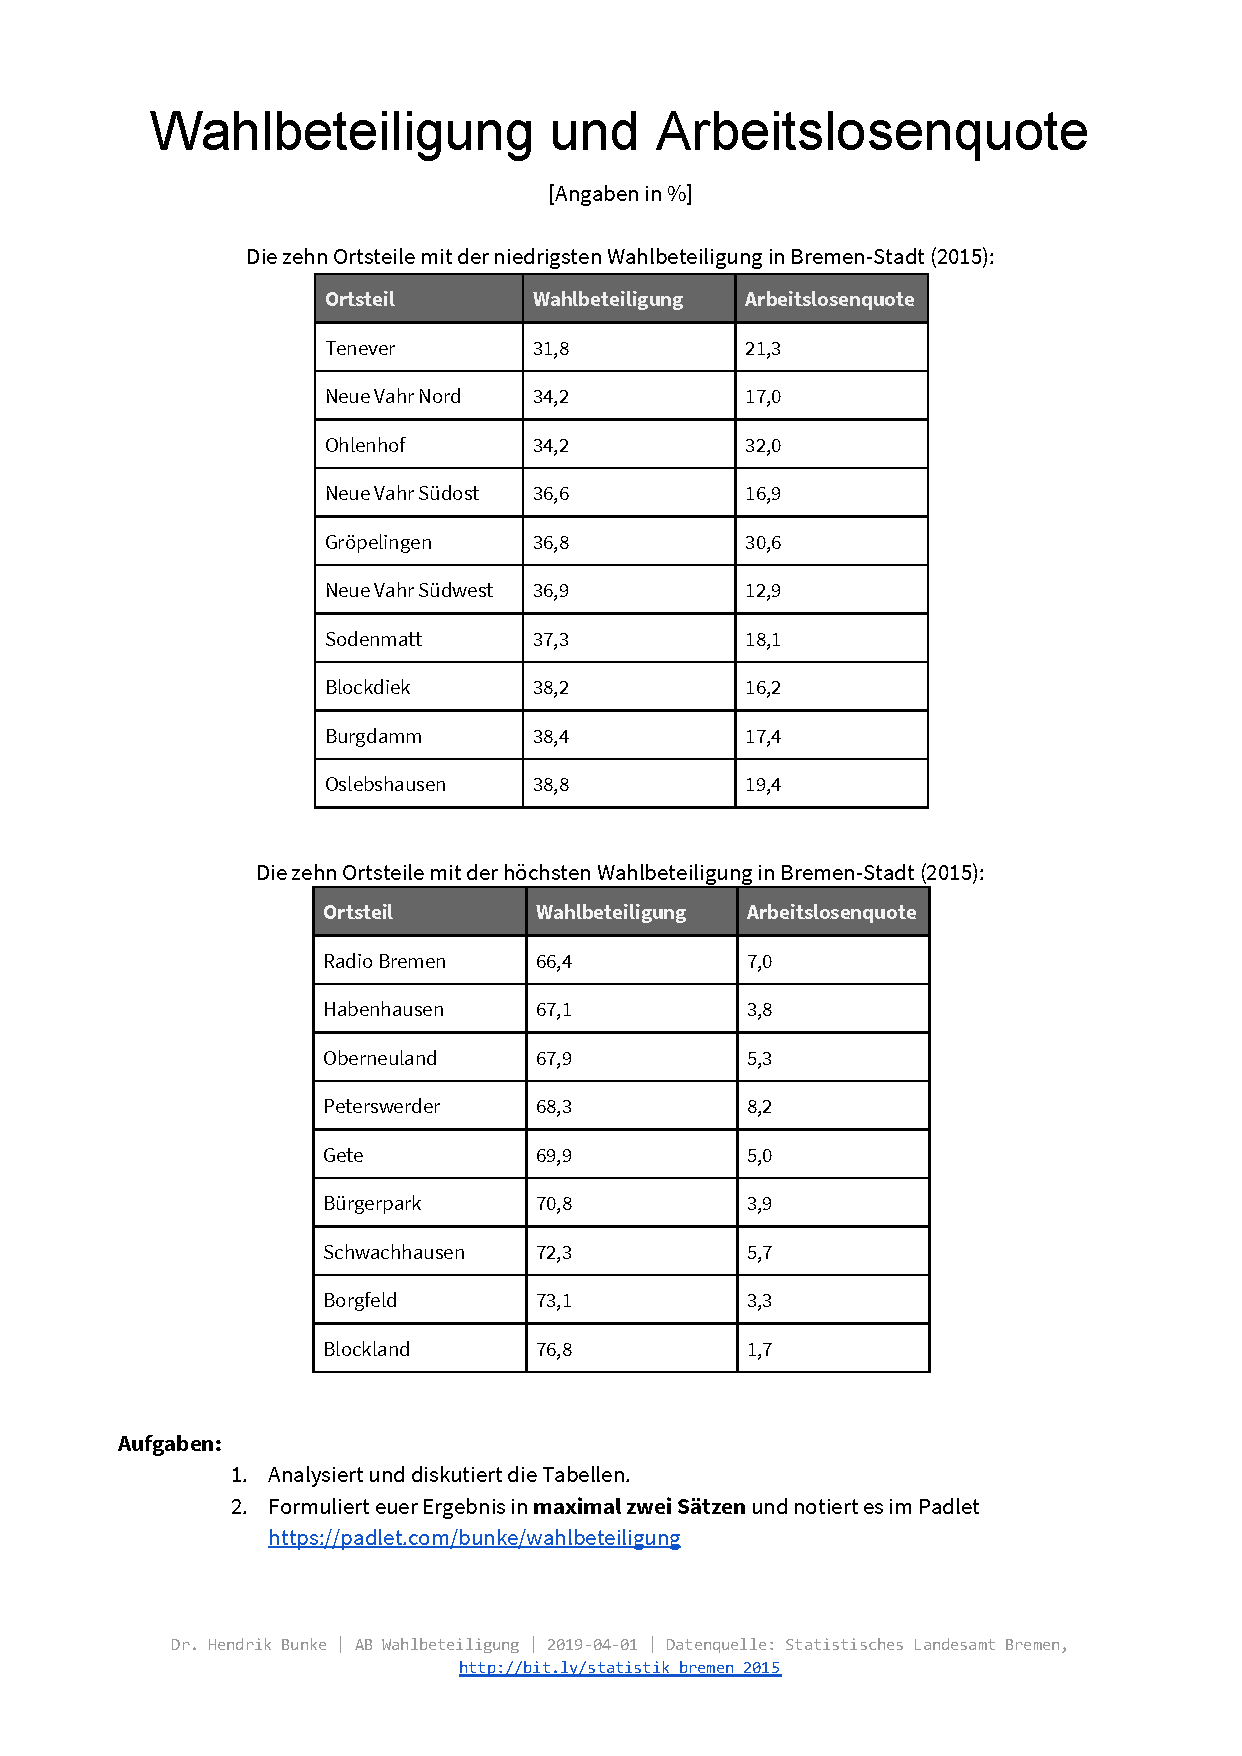
\includepdf[pages=-]{arbeitsblaetter.pdf}

\includepdf[pages=-]{praesentation.pdf}
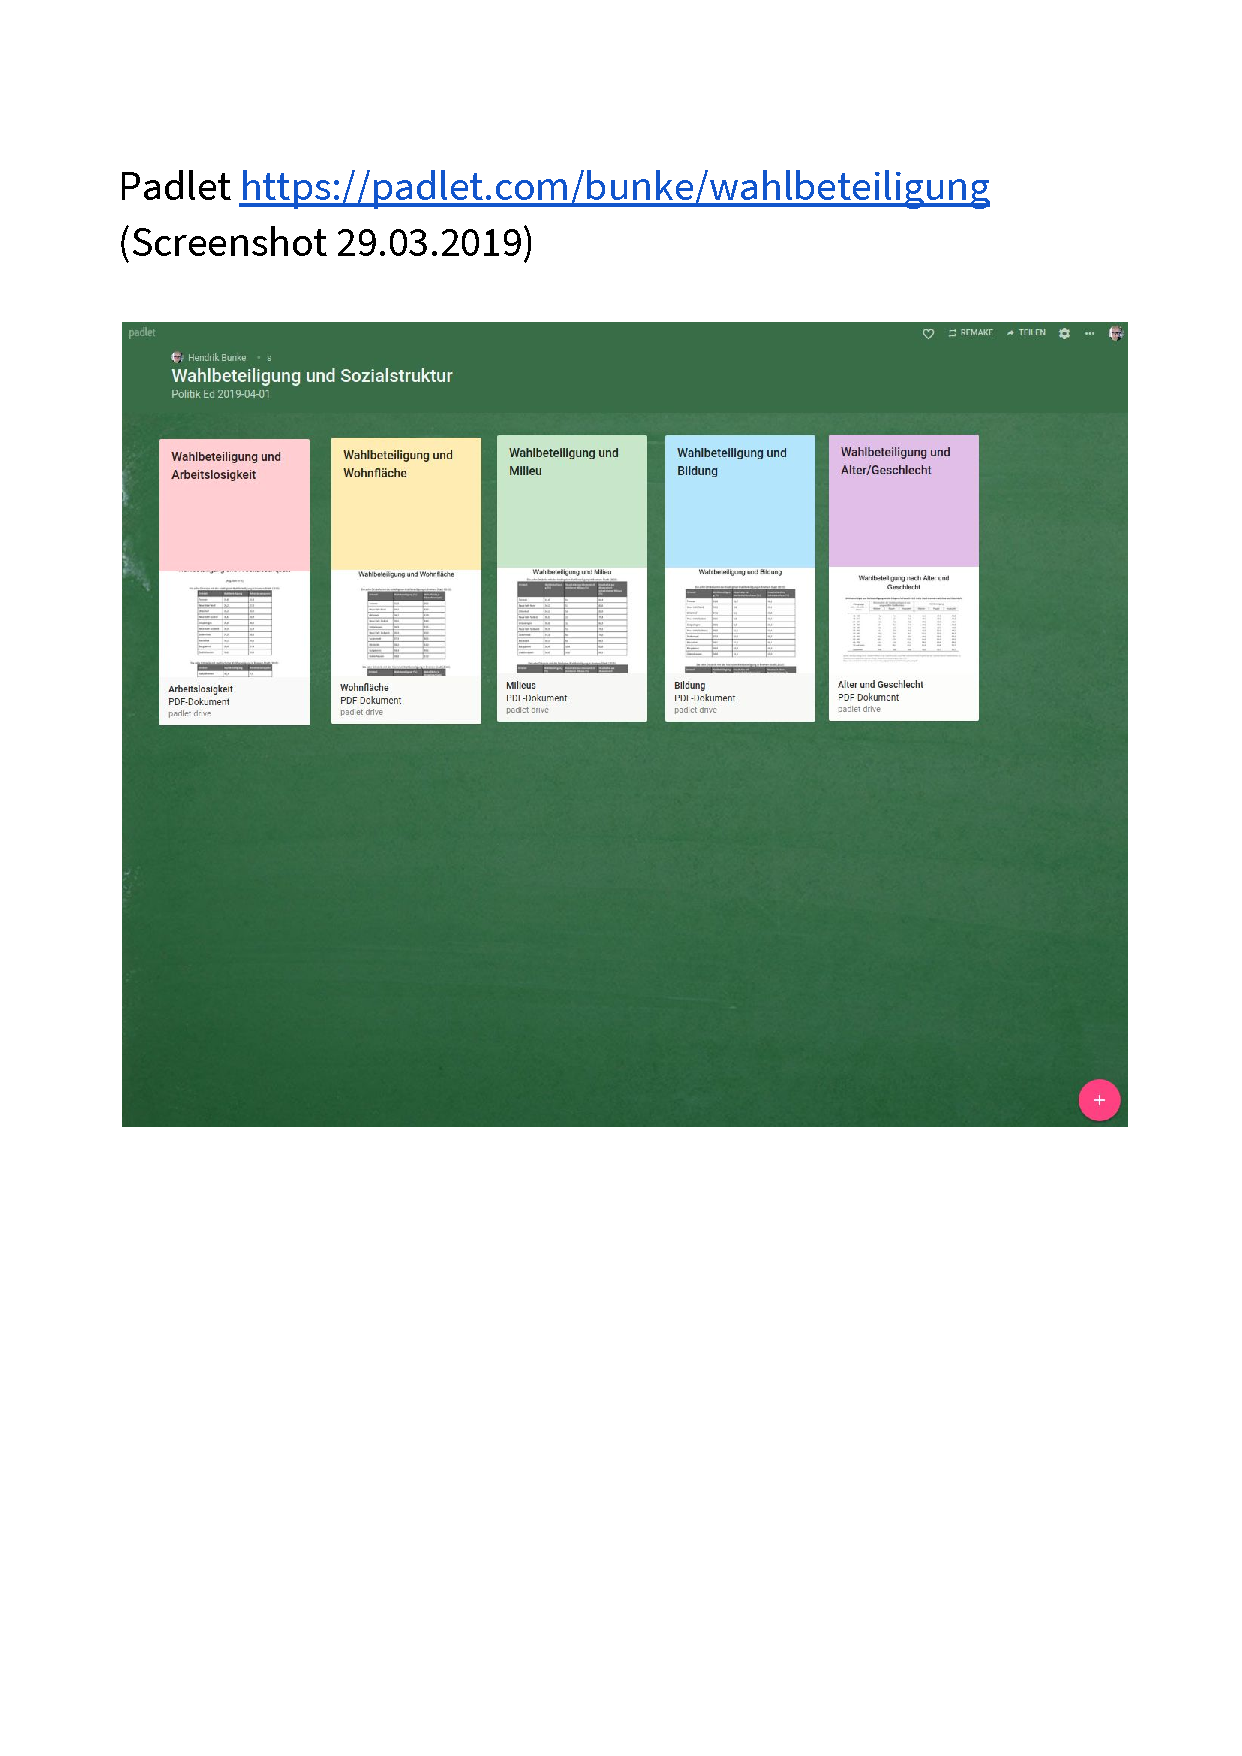
\includepdf[pages=-]{padlet.pdf}
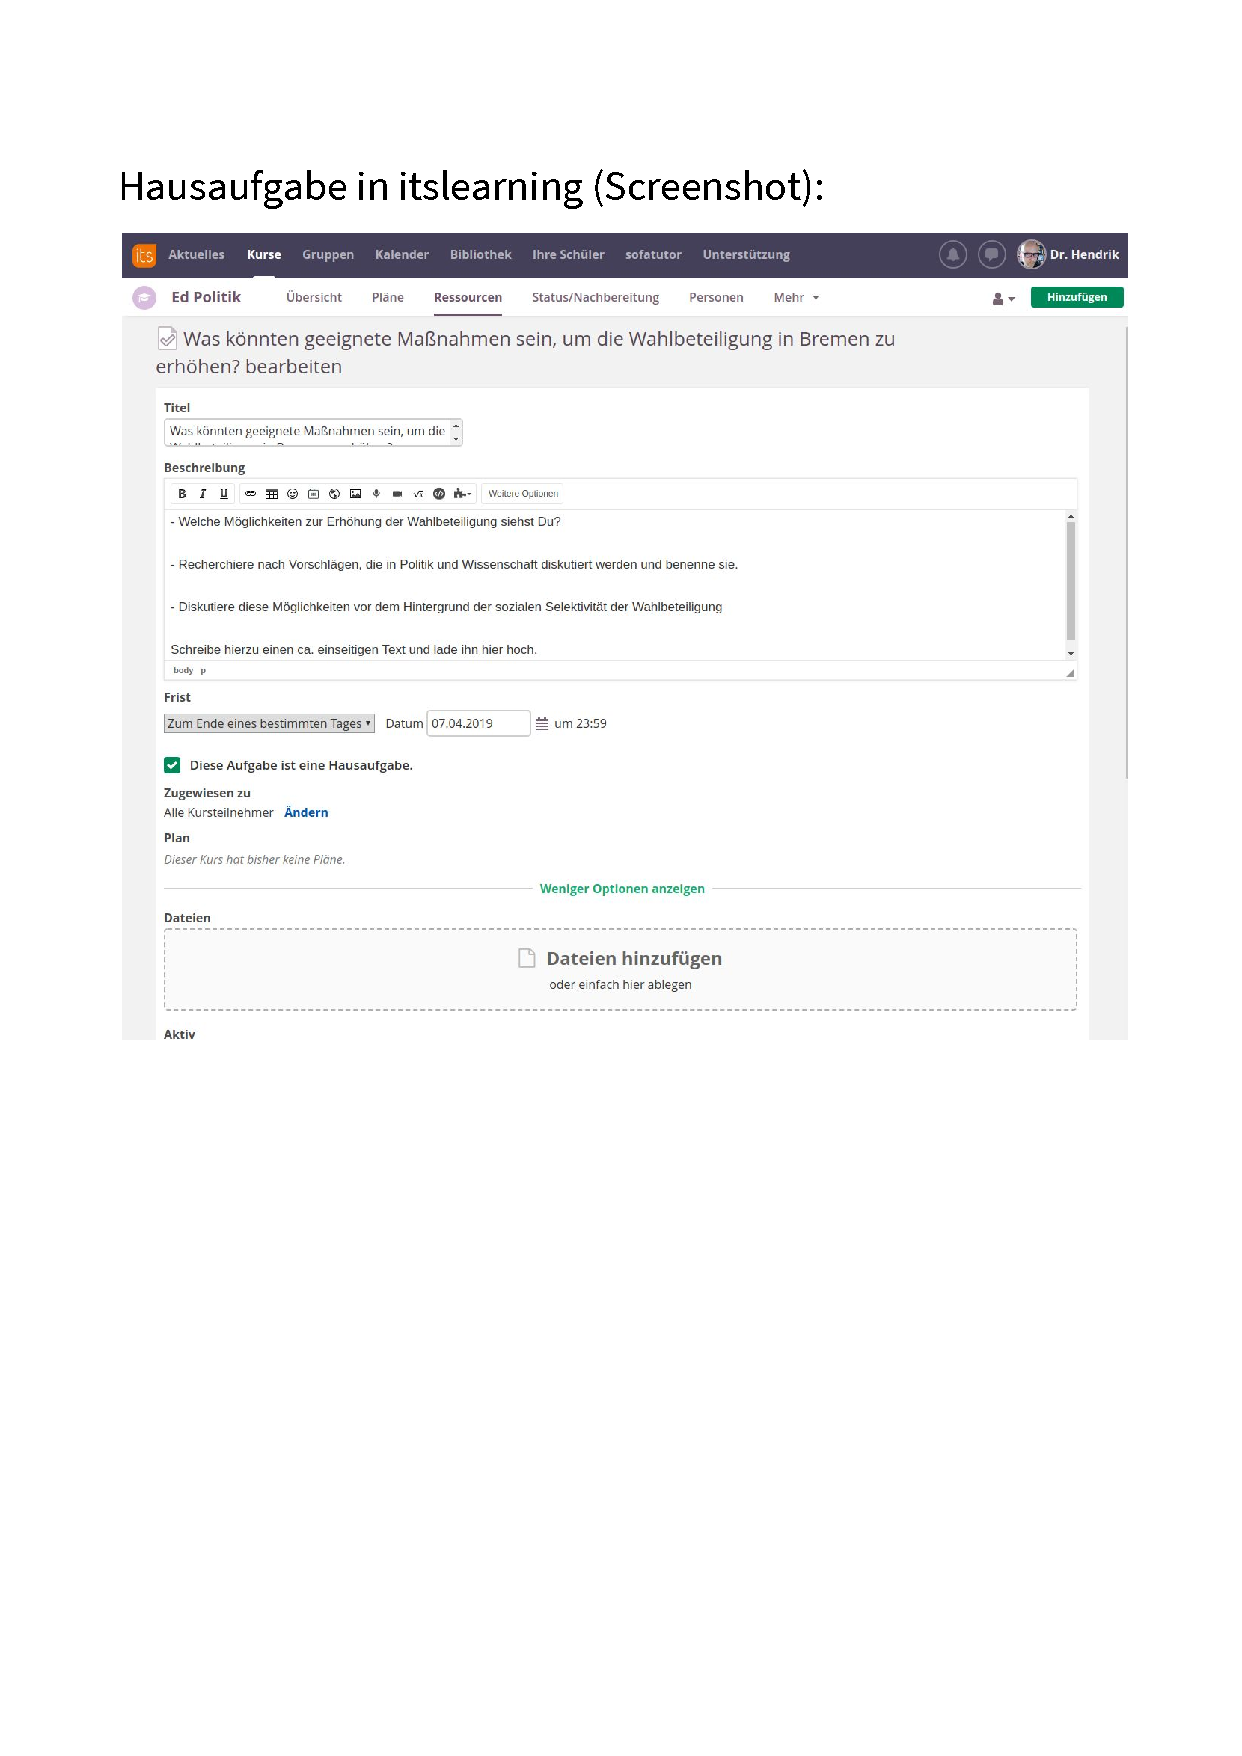
\includepdf[pages=-]{hausaufgabe.pdf}


\end{document}
